\documentclass[hidelinks,11pt,dvipsnames]{article}
% xcolor commonly causes option clashes, this fixes that
\PassOptionsToPackage{dvipsnames,table}{xcolor}
\usepackage[tmargin=1in, bmargin=1in, lmargin=0.8in, rmargin=1in]{geometry}

%%%%%%%%%%%%%%%%%%%%%%%%%%%%%%%%%%%%%%%%%%%%%%%%%%%%%%%%%%%%%%%%%%%%
%%% For inkscape-figures
%%% Assumes the following directory structure:
%%% master.tex
%%% figures/
%%%     figure1.pdf_tex
%%%     figure1.svg
%%%     figure1.pdf
%%%%%%%%%%%%%%%%%%%%%%%%%%%%%%%%%%%%%%%%%%%%%%%%%%%%%%%%%%%%%%%%%%%%
%\usepackage{import}
\usepackage{pdfpages}
\usepackage{transparent}

\newcommand{\incfig}[2][1]{%
    \def\svgwidth{#1\columnwidth}
    \import{./figures/}{#2.pdf_tex}
}

\pdfsuppresswarningpagegroup=1

% enable synctex for inverse search, whatever synctex is
\synctex=1
\usepackage{float,macrosabound,homework,theorem-env}
\usepackage{microtype}


% font stuff
\usepackage{sectsty}
\allsectionsfont{\sffamily}
\linespread{1.1}

% bibtex stuff
\usepackage[backend=biber,style=alphabetic,sorting=anyt]{biblatex}
\addbibresource{main.bib}

% colored text shortcuts
\newcommand{\blue}[1]{\color{MidnightBlue}{#1}}
\newcommand{\red}[1]{\textcolor{Mahogany}{#1}}
\newcommand{\green}[1]{\textcolor{ForestGreen}{#1}}


% use mathptmx pkg while using default mathcal font
\DeclareMathAlphabet{\mathcal}{OMS}{cmsy}{m}{n}

% fixes the positioning of subscripts in $$ $$
\renewcommand{\det}{\operatorname{det}}

\usetikzlibrary{positioning, arrows.meta}
\newcommand{\here}[2]{\tikz[remember picture]{\node[inner sep=0](#2){#1}}}

%%%%%%%%%%%%%%%%%%%%%%%%%%%%%%%%%%%%%%%%%%%%%%%%%%%%%%%%%%%%%%%%%%%%%
%%% Entry Counter
%%%%%%%%%%%%%%%%%%%%%%%%%%%%%%%%%%%%%%%%%%%%%%%%%%%%%%%%%%%%%%%%%%%%%
\newcounter{entry-counter}
\newcommand{\entry}[1]
{
	\addtocounter{entry-counter}{1}
    \tchap{Entry \arabic{entry-counter}}
	%\addcontentsline{toc}{section}{Entry \arabic{entry-counter}: #1}
	\vspace{-1.5em}
    \begin{center}
		\small \emph{Written: #1}
    \end{center}
}

\usepackage{titling}
\renewcommand\maketitlehooka{\null\mbox{}\vfill}
\renewcommand\maketitlehookd{\vfill\null}


\usepackage{tikz}
\usetikzlibrary{positioning,calc,intersections,through,backgrounds, shapes.geometric, decorations.markings,arrows}

\def\sset{\subseteq}
\def\iso{\cong}
\def\gend#1{\langle #1\rangle}

\newcommand{\rightoverleftarrow}{%
  \mathrel{\vcenter{\mathsurround0pt
    \ialign{##\crcr
      \noalign{\nointerlineskip}$\longrightarrow$\crcr
      \noalign{\nointerlineskip}$\longleftarrow$\crcr
    }%
  }}%
}

\newcommand\makesphere{} % just for safety
\def\makesphere(#1)(#2)[#3][#4]{%
  % Synopsis
  % \makesphere[draw options](center)(initial angle:final angle:radius)
  \shade[ball color = #3, opacity = #4] #1 circle (#2);
  \draw #1 circle (#2);
  \draw ($#1 - (#2, 0)$) arc (180:360:#2 and 3*#2/10);
  \draw[dashed] ($#1 + (#2, 0)$) arc (0:180:#2 and 3*#2/10);
}
% same thing as makesphere but places white background behind
\newcommand\altmakesphere{} % just for safety
\def\altmakesphere(#1)(#2)(#3)[#4][#5]{%
  % Synopsis
  % \makesphere[draw options](center)(initial angle:final angle:radius)
  \draw [fill=white!30] #1 circle (#2);
  \shade[ball color = #4, opacity = #5] #1 circle (#2);
  \draw #1 circle (#2);
  \draw ($#1 - (#2, 0)$) arc (180:360:#2 and 3*#2/10);
  \draw[dashed] ($#1 + (#2, 0)$) arc (0:180:#2 and 3*#2/10);
  \node at #1 {#3};
}

\begin{document}
\pagestyle{empty}
	\LARGE
\begin{center}
	Algebraic Topology Homework 2 \\
	\Large
	Isaac Martin \\
    Last compiled \today
\end{center}
\normalsize
\vspace{-2mm}
\hru

\tchap{Problems from 1.1}
\begin{homework}[e]
    \prob[\textsc{Exercise 2.}] Show that the change of basepoint homomorphism $\beta_h$ depends only on the homotopy class of $h$.
    \begin{prf}
        Let $X$ be a topological space with $x_0, x_1 \in X$ and suppose $h,g: [0,1] \to X$ are homotopic paths such that $h(0) = g(0) = x_1$ and $h(1) = g(1) = x_0$. We would like to show that $\beta_h = \beta_g$, i.e. that $h$ and $g$ both induce the same homomorphism $\pi_1(X,x_0) \to \pi_1(X,x_1)$. Change of basepoint homomorphisms are isomorphisms by Proposition 1.5 in Hatcher, so this is equivalent to showing that $\beta_h \circ \beta_g^{-1} = \beta_g^{-1}\circ \beta_h = \id$. But since $\beta_g^{-1} = \beta_{\olg}$, this is a simple calculation. For any $[f] \in \pi_{1}(X,x_0)$, we have
        \begin{align*}
            \beta_h\beta_{\overline{g}}([f]) = \beta_h([\olg \cdot f\cdot g]) = [h \cdot \olg \cdot f \cdot g \cdot \olh] = [f]
        \end{align*}
        since $h \simeq g$, and similarly
        \begin{align*}
            \beta_{\olg}\beta_{h}([f]) = \beta_{\olg}([h \cdot f\cdot \olh]) = [\olg \cdot h \cdot f \cdot \olh \cdot g] = [f].
        \end{align*}
        This means $\beta_{\olg}$ is the inverse of both $\beta_g$ and $\beta_h$, and by the uniqueness of inverses, we conclude $\beta_h = \beta_g$.
    \end{prf}
	\prob[\textsc{Exercise 5.}] Show that for a space $X$, the following three conditions are equivalent:
	\begin{itemize}
		\item[(a)] Every map $S^1 \rightarrow X$ is homotopic to a constant map, with image a point.
		\item[(b)] Every map $S^1 \rightarrow X$ extends to a map $D^2 \rightarrow X$.
		\item[(c)] $\pi_1 (X,x_0) = 0$ for all $x_0 \in X$.
	\end{itemize}
	Deduce that a space $X$ is simply-connected iff all maps $S^1 \rightarrow X$ are homotopic. [In this problem, 'homotopic' means 'homotopic without regard to basepoints.']
	\begin{prf} We prove the following chain of implications:

	\vspace{1em}
		  $(a) \implies (b):~$ Suppose that for every map $S^1 \rightarrow X$ is nullhomotopic to a function $c_{x_0} : S^1 \rightarrow X$ where $c_{x_0}(x) = x_0$, i.e. suppose there exists a homotopy $f_t:S^1 \rightarrow X$ where $f_1 = c_{x_0}$ and where $f_0$ is any map $S^1 \rightarrow X$. Since $(D^2, S^1)$ is a CW-pair, it has the homotopy extension property, and thus $f$ extends to $f': D^2 \times [0,1] \rightarrow X$ where $f'|_{S^1} = f$. Thus every map $S^1 \rightarrow X$ extends to $D^2 \rightarrow X$.
		  
		  $(b) \implies (c):~$ Suppose that $[f] \in \pi_1(X,x_0)$. $f(0) = f(1) = x_0$, meaning that we can interpret $f$ instead as a function $f:S^1 \rightarrow X$. This $f$ can be extended to a function $f': D^2 \rightarrow X$, but since $D^2$ is contractible, $f'$ is nullhomotopic. Thus, $f$ is also nullhomotopic, and $[f] = [0]$. This is true of any arbitrary $[f] \in \pi_1(X,x_0)$, and so we know that $\pi_1(X,x_0)$ is trivial. Noticing that the choice of $x_0$ was arbitrary, we conclude that $\pi_1(X) = 0$.
		  
		  $(c) \implies (a):~$This argument is very similar to the previous one. Each map $S^1 \rightarrow X$ can be interpreted as a loop in $X$, and since we assume $\pi_1(X) = 0$, every loop is homotopic to the trivial map. Thus every map $S^1 \rightarrow X$ is homotopic to a constant map in $X$.
		  
		  \bigskip
		  
		  A space $X$ is "simply connected" if and only if it is path connected and $\pi_1(X) = 0$. As we just showed, this is equivalent to "$X$ is path connected and every $S^1 \rightarrow X$ is nullhomotopic". If we interpret two maps $f,g:S^1 \rightarrow X$ as loops in $X$ with basepoints $x_0$ and $x_1$ respectively, then $f$ and $g$ are homotopic in $X$ by the homotopy that first shrinks $f$ to the constant map $c_{x_0}$, moves $x_0$ along a path to $x_1$, and finally deforms $c_{x_1}$ into $g$. Thus, any two maps $S^1 \rightarrow X$ are homotopic. We conclude that $X$ is simply connected if and only if all maps $S^1 \rightarrow X$ are homotopic.
    \end{prf}

\prob[\textsc{Exercise 6.}] We can regard $\pi_1 (X,x_0)$ as the set of basepoint-preserving homotopy classes of maps $(S^1,s_0) \rightarrow (X,x_0)$. Let $[S^1,X]$ be the set of homotopy classes of maps $S^1 \rightarrow X$ with no conditions on basepoints. Thus there is a natural map $\Phi: \pi_1(X,x_0) \rightarrow [S^1,X]$ obtained by ignoring basepoints. Show that $\Phi$ is onto if $X$ is path-connected, and that $\Phi([f]) = \Phi([g])$ iff $[f]$ and $[g]$ are conjugate in $\pi_1(X,x_0)$. Hence $\Phi$ induces a one-to-one correspondence between $[S^1,X]$ and the set of conjugacy classes in $\pi_1(X)$, when $X$ is path-connected. 

\begin{prf}
We first show that $\Phi$ is onto. Let $[f]$ be a member of $[S^1, X]$. Since every map $S^1 \rightarrow X$ can be regarded as a loop in $X$, $f$ is a loop based at some point $x_1 \in X$. Because $X$ is path connected, there must be some path $\gamma$ from $x_1$ to $x_0$. The map $g = \gamma \cdot f \cdot \overline{\gamma}$ is a continuous path that begins and ends at $x_0$, and is therefore a loop around $x_0$. Since $f$ and $g$ are homotopic, $[g] = [f]$. Since $[g] \in \pi_1(X,x_0)$, $\Phi([g]) = [f]$. We conclude that $\Phi$ is surjective. 

\bigskip

We now show that $\Phi([f]) = \Phi([g])$ if and only if $[f]$ and $[g]$ are conjugates. We show the forward implication first.

Assume that $\Phi([f]) = \Phi([g])$. This means that $f$ and $g$ are in the same equivalence class of $[S^1, X]$, so there must exist a homotopy $\varphi : S^1 \times [0,1] \rightarrow X$, where $\varphi_0 = f$ and $\varphi_1 = g$. The induced homeomorphisms $\varphi_{0*}$ and $\varphi_{1*}$ then satisfy $\varphi_{0*} = \beta_h \varphi_{1*}$, where $\beta_h : \pi_1(X, \varphi_1(s_0)) \rightarrow \pi_1(X, \varphi_0(s_0))$ and $h$ is the loop $\varphi_t(s_0)$. This means 

\begin{equation*}
    \varphi_{0*}([1]) = [g \cdot 1] = [g] = \beta_h\varphi_{1*}([1]) = \beta_h([f]) = [hf\overline{h}]
\end{equation*}
where $[1]$ is the equivalence class isomorphic to $1 \in \bZ$.

\bigskip

We now show the reverse implication. Assume that $[g] = [h][f][\overline{h}]$ in $\pi_1(X, x_0)$, i.e. assume $[f]$ and $[g]$ are conjugates. We want to show that $[f] = [g]$, or that $[f] = [h][f][\overline{h}]$. Consider the following function:
\begin{equation*}
    F: [0,1] \times S^1 \rightarrow X 
    \hspace{30pt}
    F_s(t) = 
    \begin{cases}
        h(3t + s) & 0 \leq t \leq \frac{1-s}{3} \\
        f\left(\frac{3}{1+2s}(t - \frac{1 - s}{3})\right) & \frac{1 - s}{3} \leq t \leq \frac{2+s}{3} \\
        \overline{h}\left(3(t - \frac{2 + s}{3})\right) & \frac{2 + s}{3} \leq t \leq 1
    \end{cases}
\end{equation*}

Since $F_0 = h \cdot f \cdot \overline{h}$, $F_1 = f$, and $F$ is continuous by the pasting lemma, $F$ is a homotopy between $f$ and $h \cdot f \cdot \overline{h}$. Thus, $[f] = [h][f][\overline{h}]$ in $[S^1, X]$ and we conclude that $\Phi([g]) = \Phi([f])$.

\end{prf}
\prob[\textsc{Exercise 10.}]From the isomorphism $\pi_1(X\times Y, (x_0,y_0)) \approx \pi_1(X,x_0) \times \pi_1(Y,y_0)$ it follows that loops in $X \times \{y_0\}$ and $Y \times \{x_0\}$ represent commuting elements of $\pi_1\left(X \times Y, (x_0,y_0)\right)$. Construct an explicit homotopy demonstrating this.

\begin{prf}
    Let $[f]$ and $[g]$ be loops based at $x_0$ in $X$ and $y_0$ in $Y$, respectively. Next consider the following homotopies:
    \begin{equation*}f_t(s) = 
        \begin{cases}
            x_0 & 0 \leq s \leq \frac{t}{2} \\
            f(2s) & \frac{t}{2} \leq s \leq \frac{1+t}{2} \\
            x_0 & \frac{1 + t}{2} \leq s \leq 1
        \end{cases}
    \end{equation*}
    and 
    \begin{equation*}g_t(s) = 
        \begin{cases}
            y_0 & 0 \leq s \leq \frac{t}{2} \\
            g(2s) & \frac{t}{2} \leq s \leq \frac{1+t}{2} \\
            y_0 & \frac{1 + t}{2} \leq s \leq 1
        \end{cases}
    \end{equation*}
Here $f_0$ is the path that transverses $f$ and then stays at $x_0$. $f_1$ is the path that stays at $x_0$ for half the interval and then transverses $f$. $g_0$ is the path that stays at $y_0$ and then transverses $g$, and finally $g_1$ is the path that transverses $g$ and then stays at $y_0$.

Next since $\pi_1(X,x_0) \times \pi_1(Y,y_0) \approx \pi(X \times Y, (x_0,y_0))$ and $h_t(s) = (f_t(s),g_t(s))$ is an element of $\pi_1(X,x_0) \times \pi_1(Y,y_0)$, then $f_0 \cdot g_0 \simeq f_1 \cdot g_1$. However, since $f_0 \cdot g_0 \simeq f \cdot g$ and $f_1 \cdot g_1 \approx g \cdot f$, we conclude that $f\cdot g \simeq g\cdot f$.
\end{prf}

\prob[\textsc{Exercise 15.}] Given a map $f:X\to Y$ and a path $h:I\to X$ from $x_0$ to $x_1$, show that $f_*\beta_h = \beta_{fh}f_*$.
\begin{prf}
    Let $[\alpha] \in \pi_1(X,x_1)$ be an arbitrary equivalence class of loops based at $x_1$. By definition,
    \begin{align*}
        f_*(\beta_h([\alpha])) = f_*[h\cdot \alpha \cdot \olh] = [f\circ (h\cdot \alpha \cdot \olh)]
    \end{align*}
    and 
    \begin{align*}
        \beta_{fh}(f_*([\alpha])) = \beta_{fh}([f\circ \beta]) = [(f\circ h)\cdot (f\circ \alpha)\cdot \ol{(f\circ h)}].
    \end{align*}
    However, up to a possible reparameterization, $(f\circ h)\cdot (f\circ \alpha)\cdot \ol{(f\circ h)}$ and $f\circ (h\cdot \alpha \cdot \olh)$ are identical paths on $Y$. In fact, if we perform concatenation from consistently, then they are identical without \emph{any} reparameterization.
    
    To see this, concatenate from right to left without loss of generality. For $t \in [0,1/2]$ we have
    \begin{align*}
      f\circ (h\cdot (\alpha\cdot \olh))(t) = f(h(t)) = (f\circ h) \cdot \big((f\circ \alpha) \cdot \ol{(f\circ h)}\big)(t),
    \end{align*}
    and we have something similar for $t \in [1/2,3/4]$ and $t \in [3/4,1]$. As the representatives of the resulting equivalence classes above are homotopic, the diagram shown by Hatcher commutes.
\end{prf}

\prob[\textsc{Exercise 16.}]$ $
\begin{enumerate}[(a)]
  \item $X = \bR^3$ with $A$ any subspace homeomorphic to $S^1$.
  \item $X = S^1 \times D^2$ with $A$ its boundary torus $S^1\times S^1$.
  \item $X = S^1\times D^2$ with $A$ the interlocked circle in the solid torus.
  \item $X = D^2 \vee D^2$ with $A$ its boundary $S^1 \vee S^1$.
  \item $X$ a disk with two points on its boundary identified and $A$ its boundary $S^1 \vee S^1$.
  \item $X$ the M\"obius band and $A$ its boundary circle.
\end{enumerate}
\begin{prf}
  \begin{enumerate}[(a)]
    \item The space $\bR^3$ contracts to the origin via the homotopy $F:\bR^3 \times I \to \bR^3$ defined $F_t(x) = (1 - t)x$, and hence has trivial fundamental group. By theorem 1.7, the circle $S^1$ has fundamental group isomorphic to $\bZ$. Therefore there exists no inclusion $\pi_1(S^1,x_0) \to \pi_1(\bR^3,x_0)$, and hence by Proposition 1.17 in Hatcher, there exists no retraction of $X$ onto a circle.

    \item In this case, we have that $\pi_1(X,x_0) \cong \bZ$ by Proposition 1.12 and $\pi_1(A,x_0) \cong \bZ\times \bZ$ by the same proposition. Note that because both of these spaces are path connected, the choice of basepoint does not matter. As any map $\bZ$-linear morphism $\bZ^2 \to \bZ$ will have nonzero kernel, there does not exist an injection $\bZ^2 \to \bZ$, and hence there is no retraction $r:A\to X$.

    \item The subset $A\subset X$ is contractible by pulling the two ends of the loops through each other. Thus, the map $\iota_*:\pi_1(A,x_0) \to \pi_1(X,x_0)$ induced by the inclusion $\iota:A\to X$ takes every loop in $A$ to something homotopic to the trivial loop in $X$. This means that the induced map $\iota_*$ is trivial, and in particular is not injective, hence by Proposition 1.17 $X$ does not retract onto $A$.
    \item Suppose we did have a retraction $r:X\to A$. In that case, the composition
      \begin{align*}
        D^2 \hookrightarrow X \xrightarrow{r} A \to S^1
      \end{align*}
      would also be a retraction. However, this is impossible, as $D^2$ is contractible while $S^1$ is not. Hence there is no such retraction $r$.
    \item 
    \item Since $X$ deformation retracts onto its central circle (a fact we used on the last homework) both $X$ and $A$ have fundamental group isomorphic to $\bZ$. Let $x_0 \in A \subset X$ be a basepoint, and choose generators $\gamma \in \pi_1(A,x_0)$ and $\lambda \in \pi_1(X,x_0)$ for the fundamental groups. The image $\iota_*([\gamma])$ of $[\gamma]$ under the map induced by the inclusion $\iota:A\to X$ is then equal to $2[\lambda]$ since traversing around the boundary circle corresponds to traversing around the central circle twice. Hence the induced map $\iota_*$ is really a map $\bZ\to \bZ$ which sends $2\mapsto 1$. This is impossible, as $2 \mapsto 1$ is not possible for such a group homomorphism as all $\bZ$-linear maps $\bZ\to \bZ$ are defined $1 \mapsto nz$ for some $n \in \bZ$. Hence, there is no retraction of $X$ onto the boundary $A$.
  \end{enumerate}
\end{prf}

\prob[\textsc{Exercise 20.}] Suppose $f_t:X\to X$ is a homotopy such that $f_0$ and $f_1$ are each the identity map. Use Lemma 1.19 to show that for any $x_0 \in X$, the loop $f_t(x_0)$ represents an element of the center of $\pi_1(X,x_0)$. [One can interpret the result as saying that a loop represents an element of the center of $\pi_1(X)$ if it extends to a loop of maps $X\to X$.]
\begin{prf}
  Let $h(t) = f_t(x_0)$ be the loop taken by $x_0$ over $f_t$. Lemma 1.19 says that
  \begin{align*}
    f_{0*} = \beta_h f_{1*}.
  \end{align*}
  For any $[g] \in \pi_1(X,x_0)$, we get that
  \begin{align*}
    [g] = f_{0*}[g] = \beta_h f_{1*}[g] = \beta_h[g] = [h] * [g] * [\olh]
  \end{align*}
  since both $f_0$ and $f_1$ are identity maps. This means that $[g]\cdot [h] = [h] \cdot [g]$. Since $g$ was chosen arbitrarily, we have that $[h]$ is in the center of $\pi_1(X,x_0)$.
\end{prf}
\newpage

\tchap{Problems from 1.2}
\prob[\textsc{Exercise 3.}] Show that the complement of a finite set of points in $\bR^n$ is simply-connected if $n \geq 3$.

\begin{prf}
  \underline{\emph{Without Van Kampen:}} ~ Let $X = \bR^n - \{p_0,...,p_m\}$ be the space obtained by removing $m$-many points from $\bR^n$, where $n \geq 3$, and let $f:S^1\to X$ be a continuous map. Denote by $x_0$ the basepoint of $S^1$. We construct an explicit homotopy between $f$ and a constant map $c:S^1 \to X$, which by problem 5, is sufficient to conclude $X$ is simply-connected.

  Our homotopy will essentially be a linear interpolation with the extra stipulation that we never come within some fixed distance of any point $p_i$. To accomplish this, we first set $r$ to be half the minimum distance between the $p_i$ and between the path $f(S^1)$ and the $p_i$, that is,
  \begin{align*}
    r = \inf \left\{\|x - p_i\| \midd x \in f(S^1) \cup \{p_0,...,p_m\}, 1\leq i\leq n\right\}\Big/~2.
  \end{align*}
  The set $f(S^1)$ is the image of a compact set under a continuous function and is hence itself compact, so the minimum of $\|x - p_i\|$ for $x \in f(S^1)$ is obtained for some $i$ and some $x$. This implies that $r$ is positive. 

  We now imagine placing closed balls of radius $r$ centered at each $p_i$. It will be useful to enumerate these, so we define $D_i = D_r^n(p_i) \subseteq \bR^n$, where $D_r(p_i)$ is the closed $n$-dimensional disk of radius $r$ centered at $p_i$. These open balls are pairwise disjoint and do not intersect the path $f(S^1)$ by the definition of $r$. In particular, it means that points within distance $r$ of $p_i$ are closer to $p_i$ than to $p_j$ for any $j \neq i$. Fix a point $P \in X \setminus \bigcup_{i = 0}^m D_i$, and additionally assume that $P$ does not lie on the line between $x_0$ and $p_i$ for any $0\leq i\leq n$.

  Choose an element $x\in S^1$ and consider the line segment between $f(x)$ and $P$ parameterized by the function $\ell_x:[0,1]\to \bR^n$, $\ell_x(t) = (1-t)f(x) + tP$. The homotopy $L:S^1\times [0,1] \to \bR^n$ defined $L(x,t) = \ell_x(t)$ is then a homotopy between $f$ and the constant map $c_P:S^1 \to \bR^n$ defined $c_p(x) = P$. Ideally, this would also be a homotopy of $f$ to $c_P$ in $X$, but the collection of line segments $\{F_x([0,1])\}_{x\in S^1}$ may intersect some of the points $p_i$. We find a homotopy from $L$ to a map $F$ whose image in $\bR^n$ is at least distance $r$ from all the $p_i$.

  Suppose the line segment between $x \in S^1$ and $P$ passes through the interior of $D_i$. We have two cases: 
  \begin{enumerate}
    \item there is some largest interval $[a,b] \in S^1$ such that $\ell_a([0,1])$ and $\ell_b([0,1])$ are both tangent to $D_i$, $a < x < b$ and $\ell_y([0,1]) \cap D_i \neq \emptyset$ (see figure \ref{fig:case1}) or
    \item $\ell_y([0,1]) \cap D_i \neq \emptyset$ for all $y \in S^1$ (see figure \ref{fig:case2}).
  \end{enumerate}
  In case (1), the intersection $L([a,b] \times [0,1]) \cap D_i$ is homotopic to a plane passing through $D_i$, and we may homotope $L$ to a new map $L'$ which runs along a sector of $S^{n-1} \cong \partial D_i$ in such a way that fixes the endpoints of each path $\ell_y[0,1]\cap D_i$ for $y\in [a,b]$. In Case (2), the intersection $L(S^1 \times [0,1])$ is homotopic to a cylinder $S^1 \times [0,1]$ (see figure \ref{fig:case2} again) and can similarly be homotoped to the boundary $\partial D_i$ via a homotopy which fixes the endpoints of the paths $\ell_y([0,1])\cap D_i$ for all $y \in S^1$. 

  We may do this for each $x \in S^1$ and each $0\leq i\leq m$. The end result is a homotopy $F:S^1\times [0,1] \to \bR^n$ which, for each $x \in S^1$, is a concatenation of linear paths in $bR^n$ and arcs along the surface of $n$-dimensional disks. Call this homotopy $F$. It is a homotopy between $f$ and $c_p$ since $F(x,0) = f(x)$ and $F(x,1) = P$, and it is a homotopy in $X$ since it avoids all points $p_0,...,p_m$.

  \bigskip

  \underline{\emph{With Van Kampen:}} ~ I wrote a solution to this problem using Van Kampen before realizing that wasn't allowed. Here's that solution too -- I couldn't bear deleting it because it includes a pretty tikz picture.
Let $\{x_1,...,x_k\}$ be a finite collection of points in $\bR^n$. We can place a ${n-1}$ sphere around every point removed from $\bR^n$, ensuring that the radius is small enough to contain only one "hole", and connect every sphere with another via a straight path. Call this space $X$. Just as $\bR^n$ with a single point removed deformation retracts to $S^{n-1}$, I claim that $\bR^n - \{x_1,...,x_k\}$ deformation retracts onto $X$. Every point inside of one of the spheres retracts onto the sphere, and choosing to map every point in $\bR^n$ that is not in $X$ onto the nearest point in $X$ retains continuity. 

Every path-connected open set on this surface has the trivial fundamental group, so by Van Kampen's theorem, the fundamental group of $X$ is also trivial. Since $\bR^n - \{x_1,...,x_k\}$ deformation retracts onto $X$, we conclude that $\pi_1(\bR^n - \{x_1,...,x_k\}) = [1]$. 
\end{prf}
\bigskip
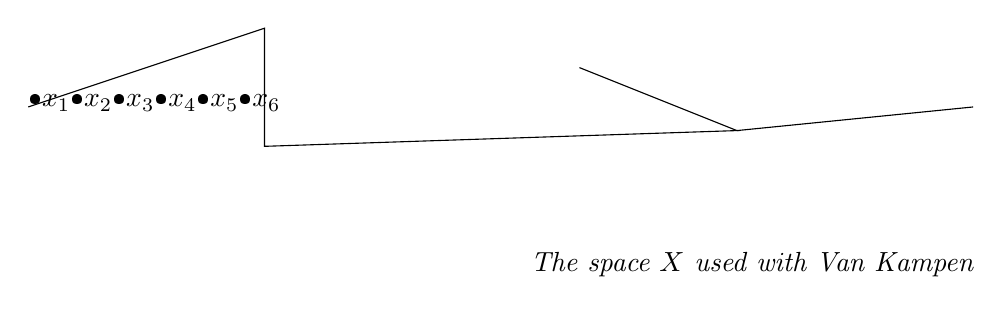
\begin{tikzpicture}
  \coordinate (A) at (15:0.5cm);
  \coordinate (B) at (3,1);
  \coordinate (S1) at (0,0);
  \coordinate (S2) at (3,1);
  \coordinate (S3) at (3,-0.5);
  \coordinate (S4) at (9,-0.3);
  \coordinate (S5) at (7,0.5);
  \coordinate (S6) at (12,0);
  \draw (S1) -- (S2) -- (S3) -- (S4) -- (S5);
  \draw (S4) -- (S6);
  \altmakesphere((S1))(0.7)(\textbullet $x_1$)[gray!10][0.4]
  \altmakesphere((S2))(0.45)(\textbullet $x_2$)[gray!10][0.4]
  \altmakesphere((S3))(0.8)(\textbullet $x_3$)[gray!10][0.4]
  \altmakesphere((S4))(0.75)(\textbullet $x_4$)[gray!10][0.4]
  \altmakesphere((S5))(0.6)(\textbullet $x_5$)[gray!10][0.4]
  \altmakesphere((S6))(0.6)(\textbullet $x_6$)[gray!10][0.4]
  \node [] at (6,-2) {\emph{The space $X$ used with Van Kampen}};
\end{tikzpicture}
\newpage
\begin{figure}[h]
    \centering
    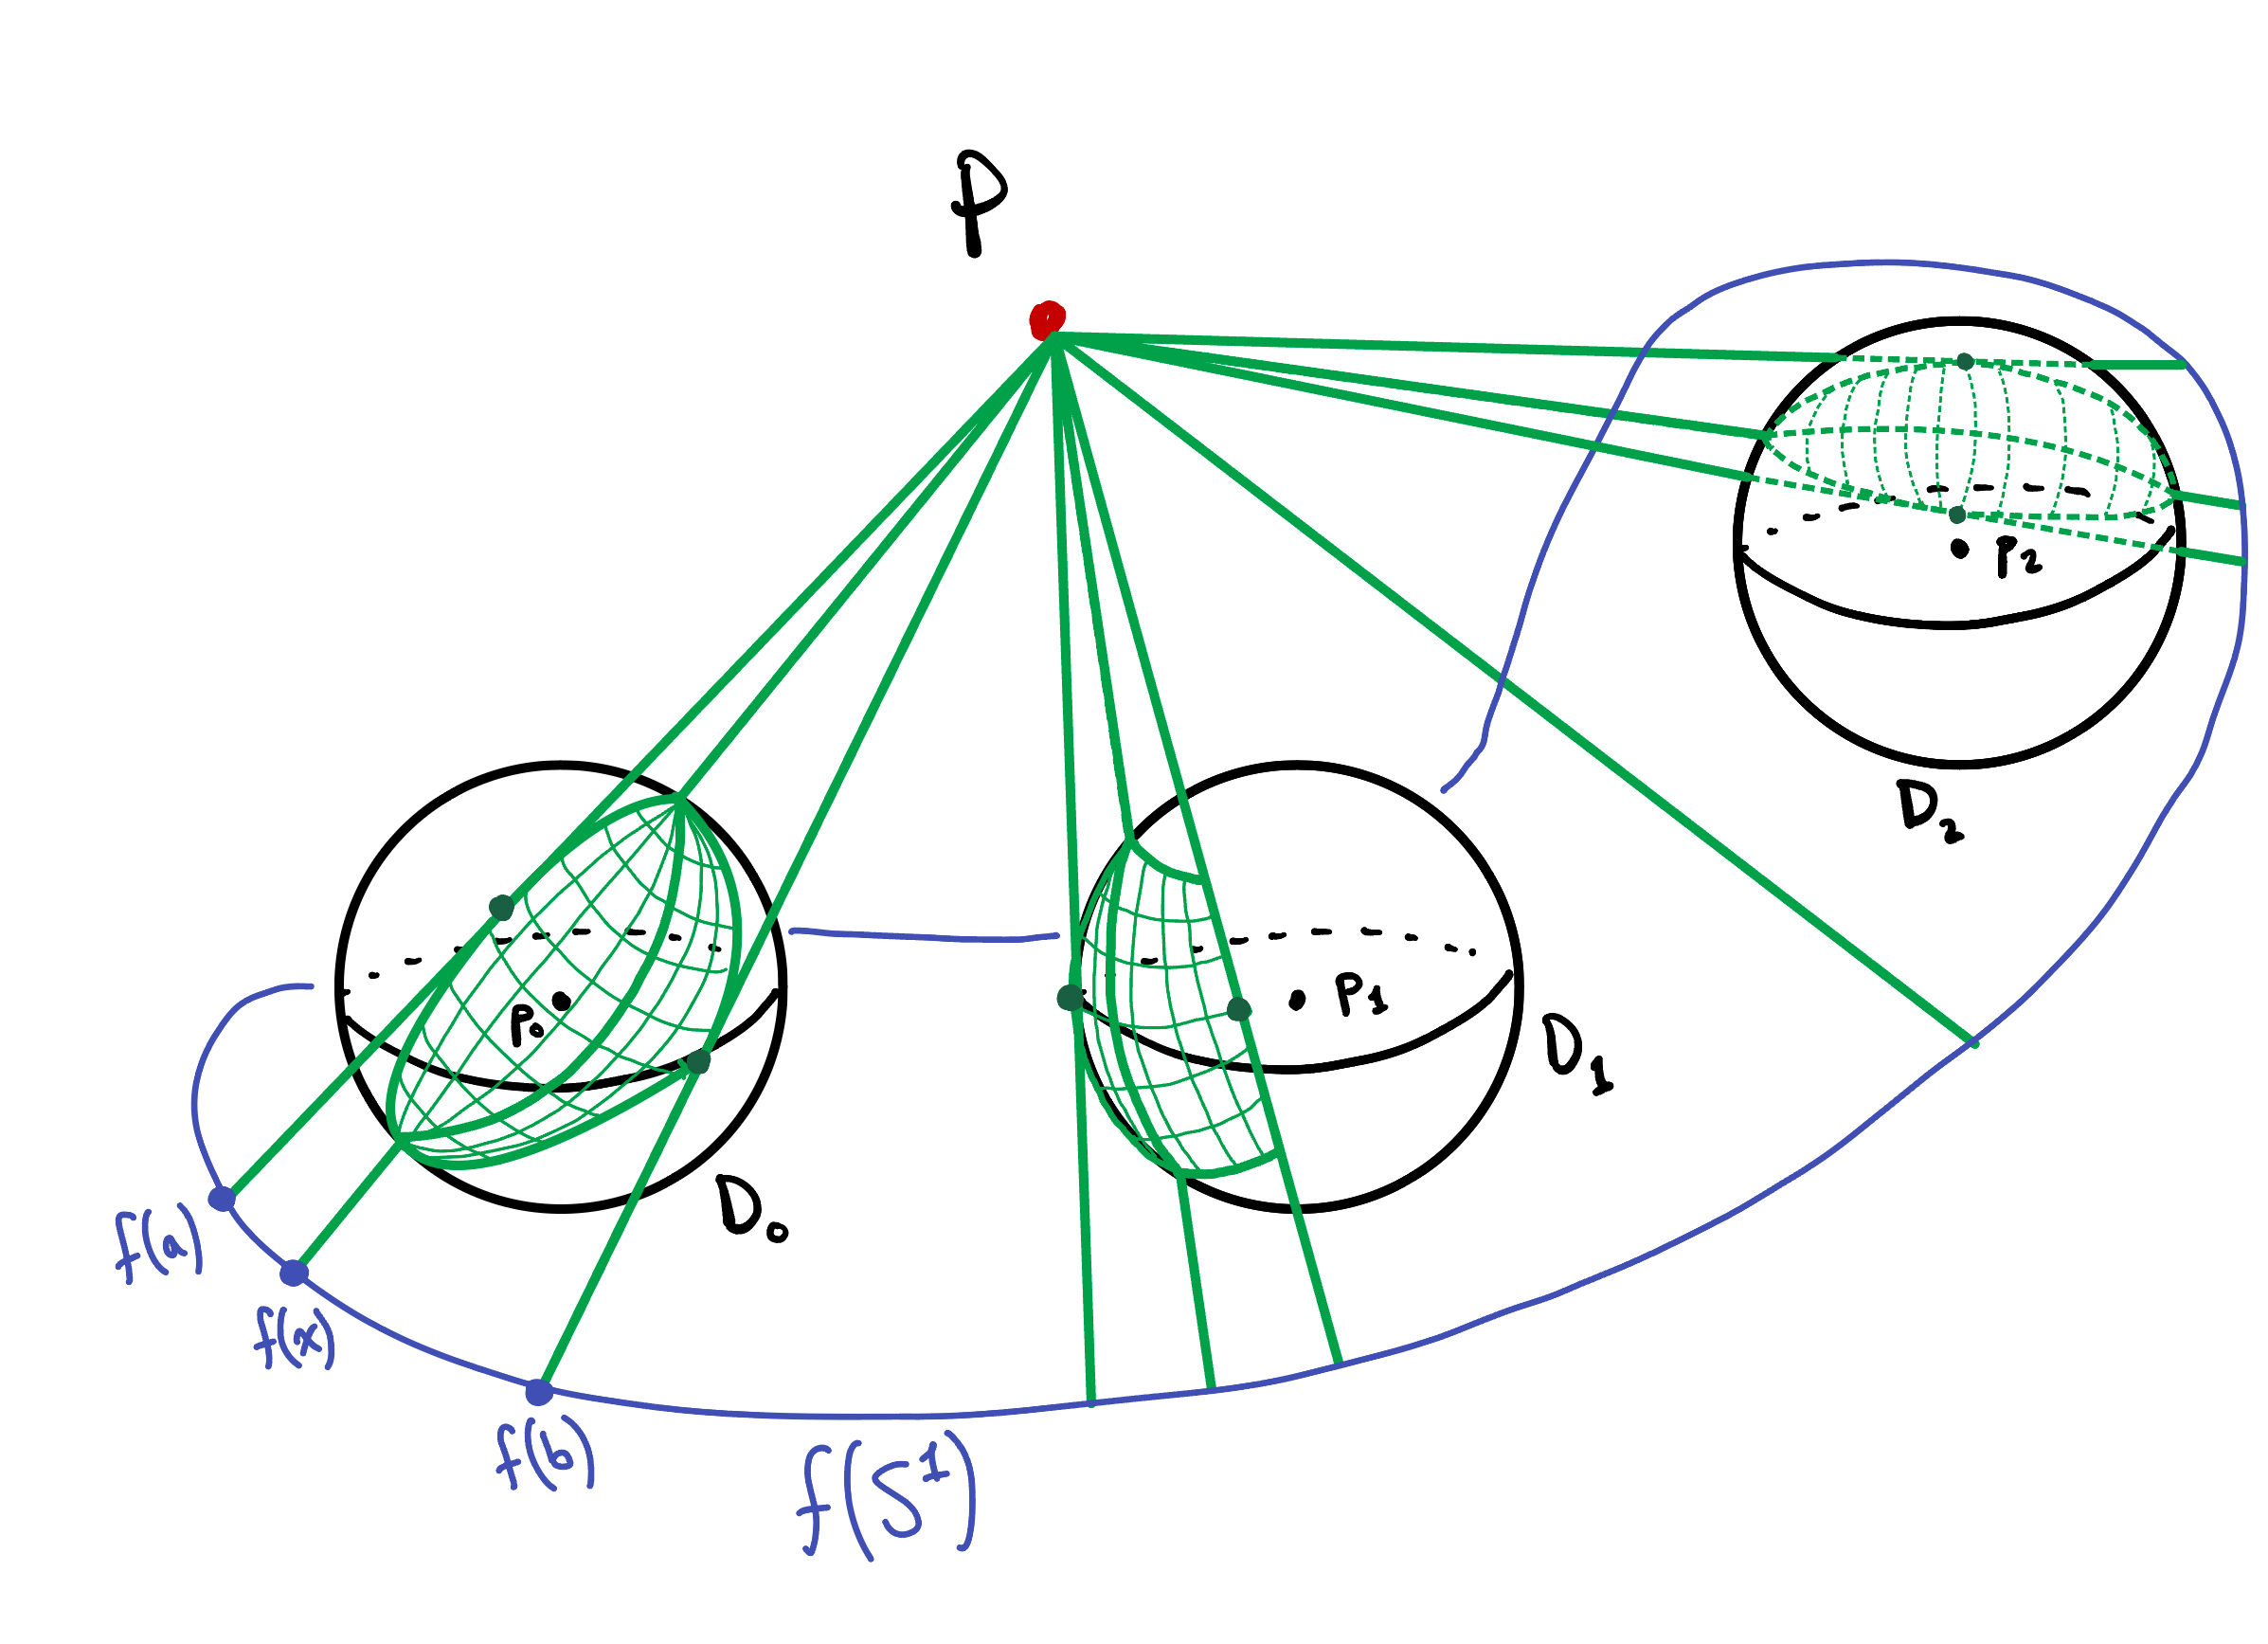
\includegraphics[width=10cm]{./figures/hwk2-fig1.jpg}
    \caption{The homotopy in Case 1}
    \label{fig:case1}
\end{figure}
\begin{figure}[h]
    \centering
    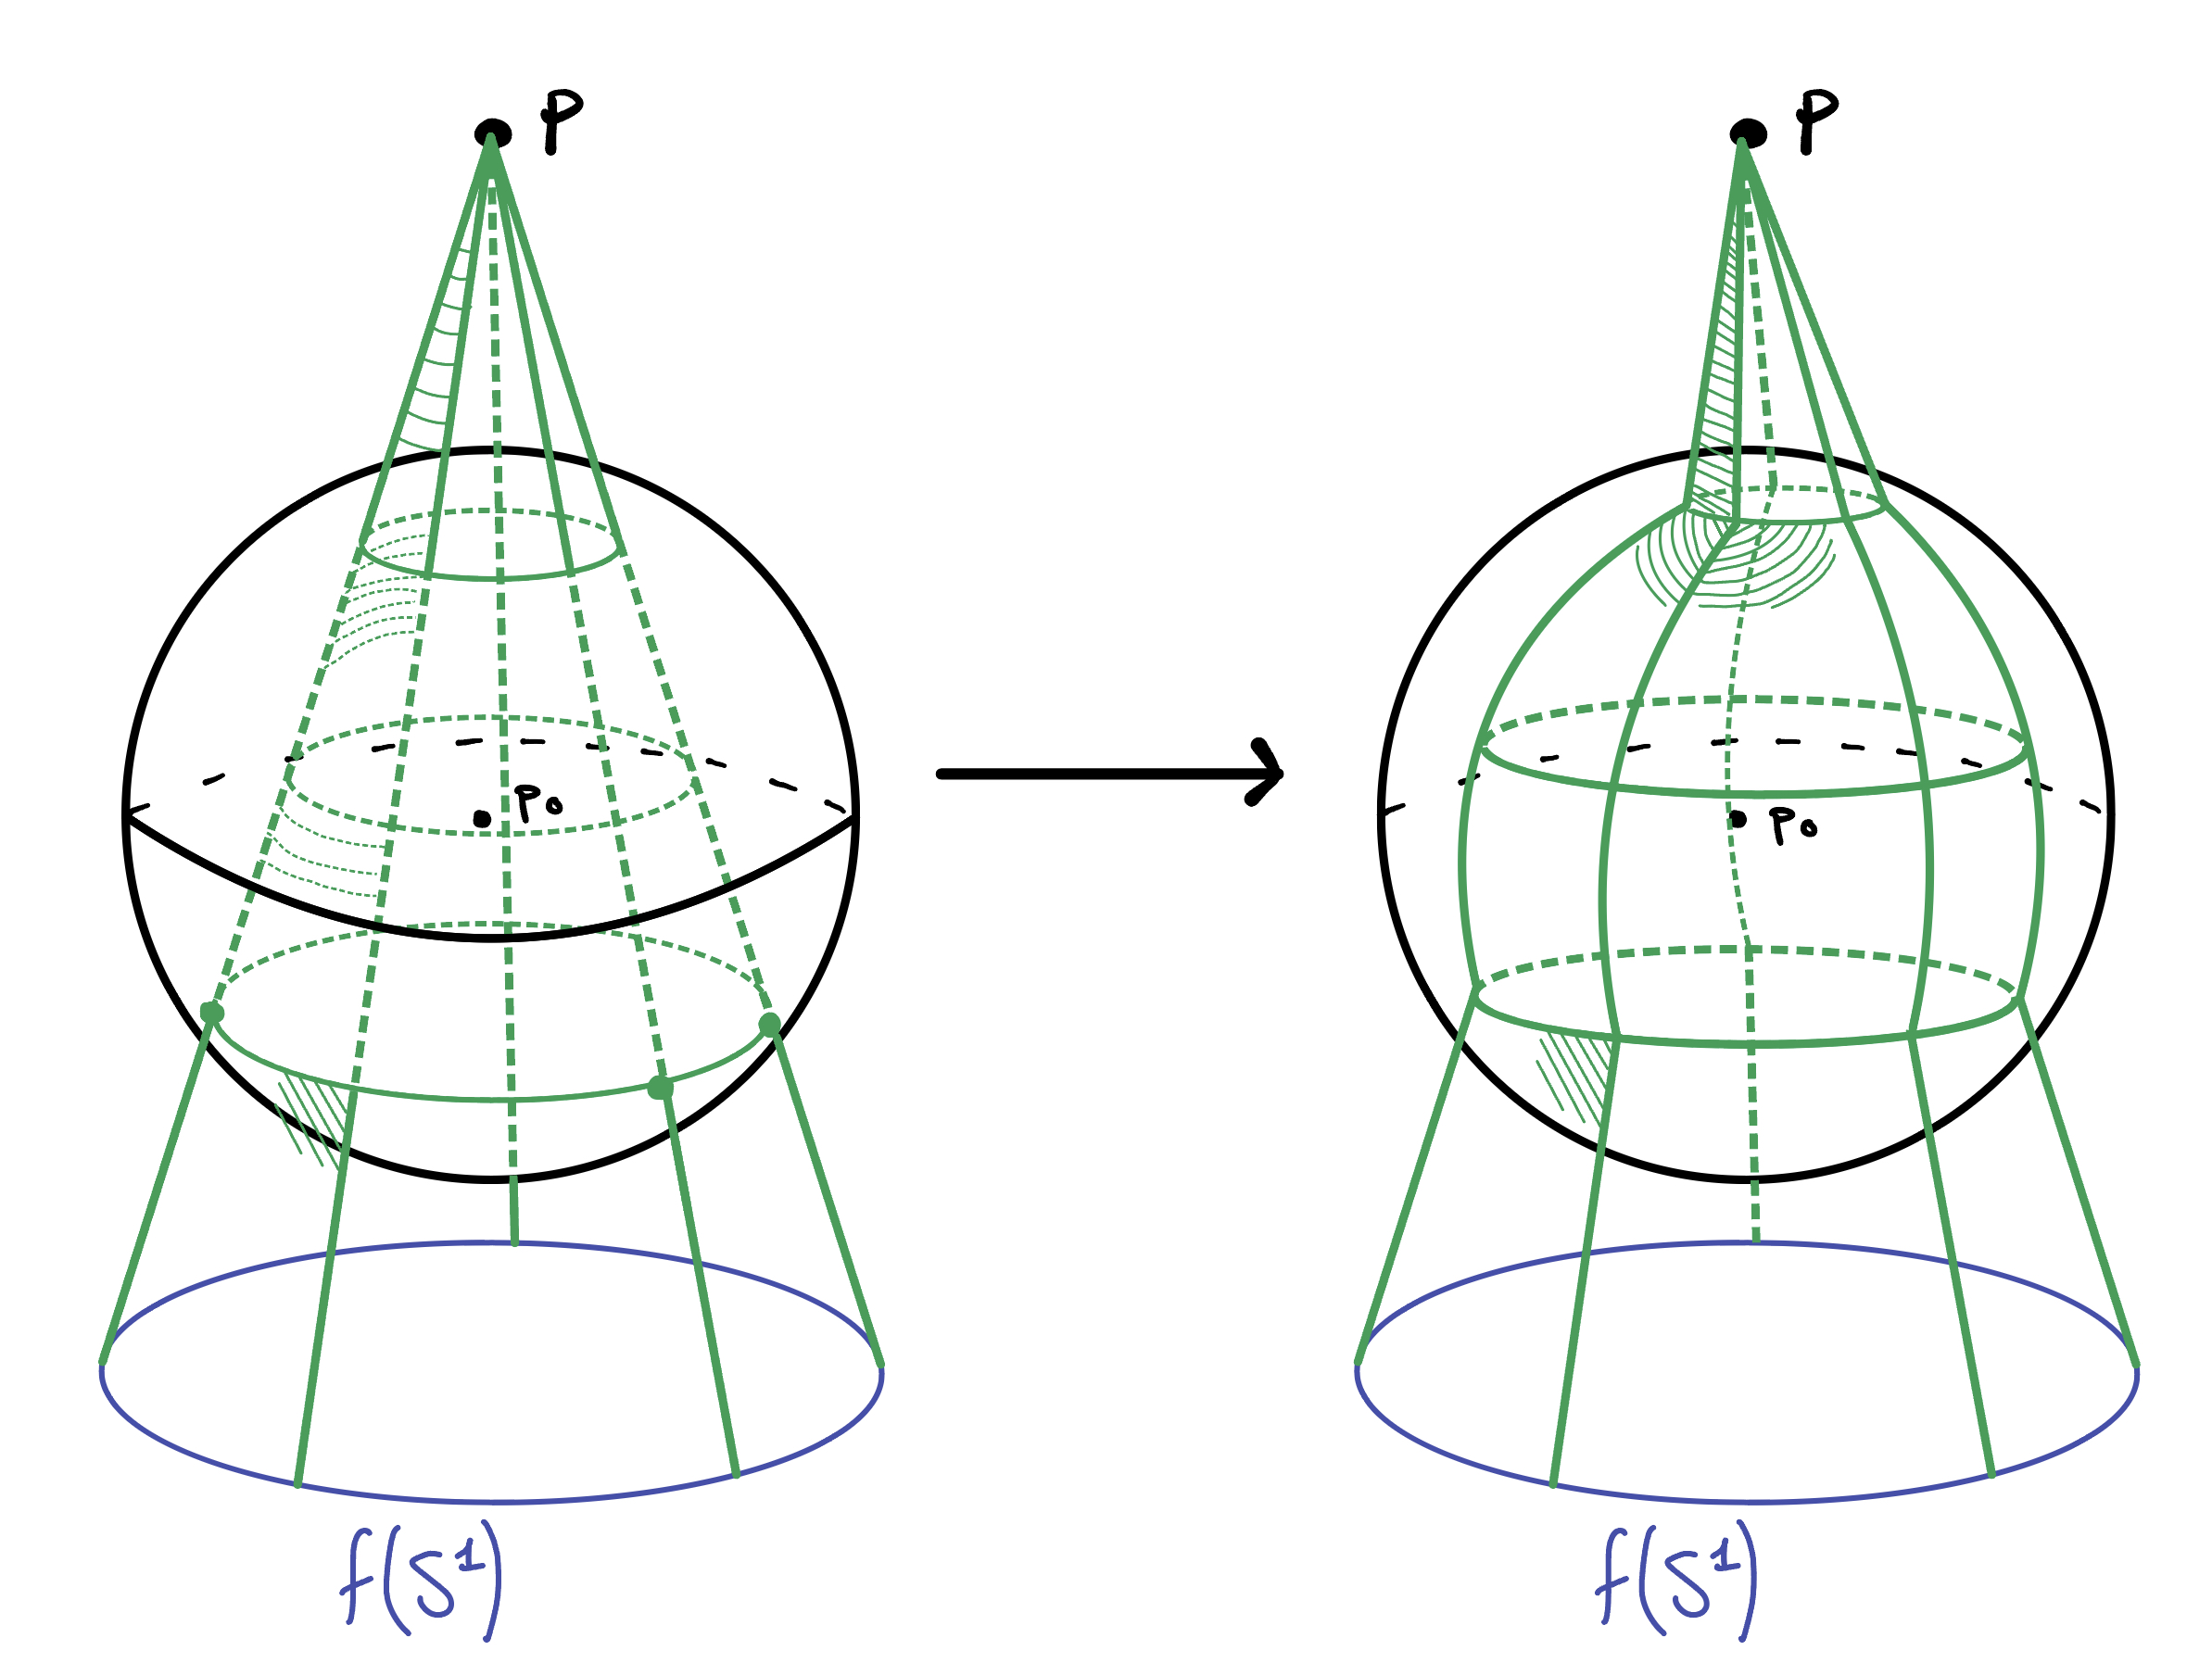
\includegraphics[width=10cm]{./figures/hwk2-fig3.jpg}
    \caption{The homotopy in Case 2}
    \label{fig:case2}
\end{figure}

\newpage

\prob[\textsc{Bonus Exercise: A ``Bad'' Group Action.}] Let $X = \bR^2 - \{0\}$. Let $G$ be the group of homeomorphisms of $X$ generated by the transformation $(x,y) \mapsto (2x,y/2)$. Let $Y$ be the quotient space $X/G$.
\begin{enumerate}[(a)]
  \item Prove that every orbit is discrete. This is meant as a stepping stone to the more general result (b).
  \item Prove that $G's$ action on $S$ is what Hatcher calls a covering space action (pg. 72).
  \item Prove that $Y$ is a manifold, except for the fact that it is \emph{not} Hausdorff.
\end{enumerate}
\begin{prf}
  \begin{enumerate}[(a)]
    \item Fix a point $p = (x,y) \in X$. For any $h \in \bZ$, we have that $g^n(x,y) = \left(2^nx,y/x^n\right)$, and hence
  \begin{align*}
    \|p - g^np\|^2 &= (x - 2^nx)^2 + (y - \frac{1}{2}y)^2 \\
                           &= x^2\left(1 - 2^n\right)^2 + y^2\left(1 - \frac{1}{2^n}\right)^2 \\
                           &> \frac{x^2}{4} + \frac{y^2}{4} = \frac{\|p\|^2}{4}.
  \end{align*}
  If we set $r = \min\left\{\frac{\|p\|^2}{4}, \|p\|\right\}$ then $g^np \not\in B_r(p)$. Thus, for any point in $X$, no point of its orbit comes within distance $r$, and hence the orbits of $X$ under $G$ are discrete.

  \item Note that, because $g$ is a homeomorphism, $g^n(U) \cap g^m(U) = \emptyset$ if and only if $g^{n - m}(U) \cap U = \emptyset$. Let $r_p = \min\left\{\frac{\|p\|^2}{8},\|p\|\right\}$. For $p \in X$ and any two points $x,y \in B_r(p)$, we have that $\|x - y\| < \frac{\|p\|}{4}$ by the triangle inequality. Hence, by part (a), all the images $g\cdot B_r(p)$ are disjoint from $B_r(p)$, and the action of $G$ upon $X$ satisfies what Hatcher calls a covering space action.

  \item Let $[p] \in X/G$ and let $B_r(p)$ be the ball of radius $r$ centered at $p \in X$ from part (b). Because $g^n B_r(p) \cap g^mB_r(p) = \emptyset$ for each $n,m \in \bZ$, the projection map $\pi:X\to X/G$ is a homeomorphism on $B_r(p)$ and $U = \pi(B_r(p))$ is an open neighborhood of $[p]$ in $X/G$. Since
    \begin{align*}
      \|p - 0\| = \|p\| \geq \min\left\{\frac{\|p\|^2}{8},\|p\|\right\} = r,
    \end{align*}
    $0 \not\in B_r(p)$ and hence $B_r(p)$ is an open disk in $\bR^2$. The inverse of the restriction $\pi|_{B_r(p)}$ then yields a homeomorphism $g:U\to B_r(p)$, so $X/G$ is locally homeomorphic to $\bR^2$.

    I do not know why $X/G$ fails to be Hausdorff, but I imagine it has something to do with the fact that the origin is a limit point of the orbit of any point of the form $(x,0),(0,y) \in X$.
\end{enumerate}
\end{prf}

\end{homework}
\end{document}
